\section{Backgrounds}
The growing dependence on information technology has led to an increased need for server rooms in various industries. Server rooms house the critical infrastructure needed to support the growing demand for data storage and processing. However, maintaining a server room can be a complex and challenging task. The performance of servers can be affected by several factors, such as temperature, humidity, dust, water leakage, voltage, and current. These factors can cause damage to the servers, leading to downtime and loss of critical data. Therefore, it is crucial to monitor the server room's environment to ensure that it is operating efficiently and reliably.\\

In recent years, advancements in sensor technology have made it easier to collect data on environmental variables within the server room. The data collected can provide insight into the server room's performance, enabling quick identification of issues before they become critical. However, managing and analyzing the data collected from sensors can be a daunting task. Therefore, there is a need for a comprehensive monitoring system that can efficiently collect, manage, and analyze data on environmental variables within a server room. In the following sections some of these difficulties are going to be discussed.
\subsection{Related Works}
Based on the article\cite{kurniawan2019smart}, it was argued that two of the factors that needed to be monitored in a server room were temperature and humidity. Therefore, in this implementation a Wemos DHT Shield wireless sensor was utilized to collect this data so the users would be able to access the real-time data on a web server hosted on a raspberry pi. In addition to that there was a notification system implemented in this system so when certain events happened it would send a message to the defined users via whatsapp. For example, the system would notify the administrator when humidity reaches 60 percent.\\

In another implementation provided in \cite{zohari2019server}, the fundamental parts of the hardware was DHT 11 sensor,  arduino UNO and ESPRESSO LITE and the system was designed as the figure \ref{fig:zohari2019server} shows. In this system, humidity and temperature of the environment was collected using an Arduino UNO and then was transferred to the cloud using a ESPRESSO LITE which after that would be visualized using a Thingspeak platform.\\
This system was not implemented to work as a real time data collecting system and the arduino reads the data from DHT 11 every 2 seconds and if anything unordinary happens like temperature going above 35  ° C or humidity reaches 80\% it would send the data to the cloud and it would trigger an alarm using the buzzer integrated into the system. but in ordinary situations it would only send these data every 15 seconds.\\

In \cite{khan2018internet}, some factors were introduced to monitor events such as unauthorized access, temperature and humidity fluctuations, smoke and leaks, airflow and vibrations so suitable action would be done in case of fire, earthquake, etc. In addition some saturation should be considered like when there is no internet connection or there is no power so we could get the information about the server room even in these times. Some of the solutions for this situation in this article was using an UPS and activating it automatically when there is no electricity to run the system. Also some of the previous studies were discussed in this article that can be seen in figure \ref{fig:khan2018internet_1}. In those systems one of the most common ways to connect a number of sensors together wirelessly was to use a WSN system that is considered to have some issues and challenges, which includes limited resources (e.g., processing, memory and power, etc.), security attacks.\\
All being considered in this design a raspberry pi was used as a smart object that collects sensor data in the area and connects to the system using a LORA gateway. In this implementation, the number of smart objects can be increased that can help with the scalability of the system. Using these smart objects also helps with taking appropriate action in case of a certain event and it can alarm the staff, control the air conditioning system, control UPS in case of electricity outage and so on.\\

One of the interesting views that was considered in \cite{choochaisri2011senvm}, was paying attention to cost when it comes to taking actions like lowering the temperature in a way that it wouldn’t cost us unnecessary electricity usage hence it would be a considerable feature when it comes to the small businesses that needs to work as efficient as they can to maintain their sources. This system was designed for a tropical area like Thailand where the temperature is between 23 and 30 celsius degrees so in most companies using an air conditioner was needed to reduce the temperature to below 20 ° C in order to prevent overheating in the highest  load times. But keeping the temperature this low is mostly because in those systems there was no real-time monitoring system on the temperature. In addition to that based on American Society of Heating Refrigerating and Air-Conditioning Engineers (ASHRAE), the temperature in a server room should be up to 27 ° C so In this system, a temperature sensor was placed in each rack and for implementing this system a Crossbow TelosB mote running on TinyOS 2.1 was used that is capable of collecting data about temperature, humidity and light, then these data was sent to a computer(base station) using a WSN system and serial protocol so that it could be analyzed by a Fuzzy logic and be sent to a web server. In this Fuzzy logic some policies were introduced to control the temperature of the room by manipulating the air conditioners in the room.\\
 
The article \cite{santos2019data} describes a prototype IoT solution and associated platform that was applied to a data center monitoring system. The prototype uses SH31 instead of DHT11 which has more precise values rated at ± 0.3ºC, and does not require Wi-Fi which demands a gateway near and most likely a power source for it to last more than a few months. The text also mentions that the data center could be improved with CoolDoor by CoolDoor Pty Ltd, a refrigerated rack door where the air being inputted into the racks would get chilled before entry. This could improve energy consumption caused by the HVAC and present better temperature values. The developed system makes it possible to determine anomalies and prevent future problems. The experiment proved that these anomalies are much more frequent than initially thought and they can be caused by the hardware itself as much as the outdoor environment conditions. It was also possible to determine ways to improve the party’s datacenter thermal flow by correctly managing the position of the server based on their 80 usage, since servers with expected higher usage should have more free space around them, providing better airflow and reducing the temperature gradient that represents one of the most important factors on hardware durability.\\

In this article\cite{nasution2019monitoring} they design a temperature and humidity remote monitoring system and server room using Lattepanda and ThingSpeak to data cloud the monitoring result. The system design process consists of two parts, the first is the design of hardware reading data on the sensor. The second is sending data to ThingSpeak capable of being resuscitated which can be accessed via the internet using a browser. From the results of the test, it can be seen that Lattepanda can be used to monitor temperature and humidity in the server room. The temperature and humidity can be monitored in real time (every 30 seconds) through the channels provided by ThingSpeak.\\



\begin{figure}
    \centering
    \captionsetup{type=figure}
    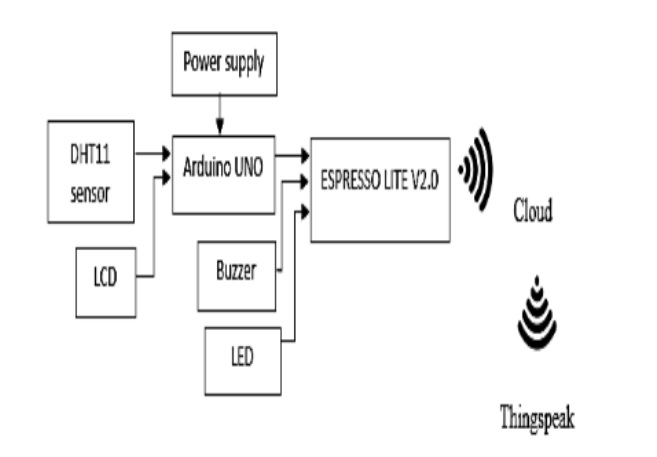
\includegraphics[width=0.7\textwidth]{zohari2019server_fig1}
    \caption{Designed system in article\cite{zohari2019server}}
    \label{fig:zohari2019server}
\end{figure}
\begin{figure}
    \centering
    \captionsetup{type=figure}
    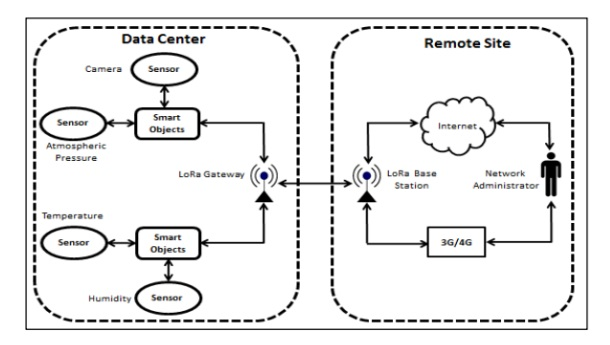
\includegraphics[width=0.7\textwidth]{khan2018internet_1}
    \caption{Designed system in article\cite{khan2018internet}}
    \label{fig:khan2018internet_1}
\end{figure}

\subsection{Monitoring the environment}
    A monitoring system should be able to monitor the environment of the server room and alert the administrators in case of any abnormality. The following list contains some of the most important parameters that should be monitored in a server room.
    \begin{itemize}
        \item Temperature
            \begin{description}
                \item Server room temperature should be maintained at a stable, suitable level to ensure the proper functioning of equipment. The recommended range of temperatures is between 18°C and 27°C \cite{ASHRAE_Storage_White_Paper_2015}.
                \begin{description}
                    \item[Too high temperature:] If the temperature inside a server room rises above the recommended range, it can cause several problems. High temperatures can make equipment operate less efficiently and potentially fail altogether. High temperatures can also decrease the life expectancy of electronic devices and increase the chance that stored data will be corrupted \cite{data_center_cooling}.
                    \item[Too low temperature:] If the temperature in a server room is allowed to fall below the recommended range, it can cause several issues. The cold air can lead to condensation—which leads directly to corrosion and equipment damage. In addition, low temperatures can decrease the efficiency of equipment and make it more likely to fail \cite{data_center_cooling}.
                \end{description}
            \end{description}
        \item Humidity
            \begin{description}
                \item On the other hand, High humidity levels can lead to condensation, which causes corrosion of the equipment and short circuits. High humidity levels can also create conditions that are conducive to the growth of mold and other microorganisms, which in turn damage equipment and affect indoor air quality \cite{10.1115/IPACK2015-48176}.
            \end{description}
        \item Dust
            \begin{description}
                \item Dust accumulation in a server room can degrade the performance and lifespan of equipment. Dust can block air vents, causing overheating, and it also attracts moisture leading to corrosion or other problems. So monitoring the levels of dust in a server room can help identifying and addressing potential problems.
                    \begin{description}
                        \item The suitable range for dust density in a server room is around 0 to 3mg/m3.
                    \end{description}
            \end{description}
        \item Water Leakage
            \begin{description}
                \item Serious consequences can result from water leakage in a server room, even if only a small amount of water leaks onto equipment. It is important to have proper monitoring systems and alerts that will notify personnel as soon as possible after any leak occurs \cite{telecommunications2010tia}.
            \end{description}
        \item Electricity
            \begin{description}
                \item Monitoring the state of electricity, including voltage and current, is important in a server room to ensure the stability and reliability of the power supply to the equipment. Electrical voltage and current fluctuations can lead to problems with electronic equipment, such as data loss and corruption. In order to minimize these risks, server rooms are typically equipped with uninterruptible power supplies (UPS) and surge protection devices that help stabilize the voltage. The following list contains some common ranges for voltage and current \cite{telecommunications2010tia}.
                \begin{description}
                    \item[Voltage:] The recommended operating range in from 208V to 240V and the maximum recommended limit is 264V.
                    \item[Current:] The recommended operating range in from 20A to 40A (per phase)
                \end{description}
            \end{description}
        \item Movement
            \begin{description}
                \item Movement sensors, also known as motion detectors, can be used in order to detect unauthorized access to the room by detecting movements within the room and alerting the administrators.
            \end{description}
        \item Smoke
            \begin{description}
                \item Smoke sensors can be used to detect smoke and alert the administrators in case of a fire.
            \end{description}
        \item Authorization
            \begin{description}
                \item Authorization devices, such as cameras, fingerprints, keypads, etc., can be used to detect unauthorized access to the room by detecting the presence of a specific person.
            \end{description}
        \end{itemize}
        \subsection{Security}
        Another aspect of a monitoring system is that it should be able to prevent any intrusions and ensure that data remains intact and that access is restricted to only those with the appropriate privileges.
        \begin{itemize}
            \item Confidentiality And Authentication
                \begin{description}
                    \item in every IOT system, a proper authentication is crucial to ensure the security of the data so it wouldn't get into the wrong hands or get mutated by malicious actors and because the data is being transmitted remotely, more security measures has to be taken \cite{saba2022anomaly,stallings2007network}.
                \end{description}
            \item Authorization
            \begin{description}
                \item Security and reliability are the most important factors in our use case of network and other security measure implementations. There are trade offs like losing flexibility but these are the trade offs that we are willing to make to reach the maximum level of security possible \cite{saba2022anomaly,stallings2007network}.
            \end{description}
        \item Integrity
            \begin{description}
                \item In an IOT system, there is a risk of intruders attempting to impersonate legitimate users and alter or manipulate data. So it is important to implement verification and encryption methods to make sure in an event of a breach, the integrity of the data is still ensured and no nefarious actor in the system can mutate or access the data in any way because the consequences can be quite catastrophic \cite{saba2022anomaly,stallings2007network}.
            \end{description}
        \end{itemize}
        \subsection{Real-time monitoring}
        Real-time monitoring is important in a monitoring system to ensure that the administrators are notified as soon as possible in case of any abnormality.
        \subsection{Data Visualization}
        Data visualization is an important part of a monitoring system, because it can provide a clear and compact representation of the data sent by the sensors. This allows administrators to quickly and easily identify trends, patterns, and anomalies in the server room environment, such as changes in temperature, humidity, power, and other environmental factors.\\
        Data visualization can be achieved through a variety of means, such as graphs, charts, and maps. These visual representations can provide a lot of information in real-time, allowing administrators to make informed decisions about the state of their server room and respond quickly to any issues or problems. For example, graphs can be used to track trends over time.

        \section{Purpose}
            The purpose of this thesis is to demonstrate how an effective and efficient monitoring system can be implemented for server rooms using sensors, which are introduced in three categories in the tables \ref{table:electrical_sensors}, \ref{table:envirement_sen} and \ref{table:security_sen}. The system will be designed to provide real-time data to a website, so that it can be monitored anywhere with internet access. This thesis will examine how this system was designed and implemented, including the selection of sensors and development of an online panel for monitoring data visualization.
            
            \begin{table}
                \centering
                \caption{Electrical sensors}
                \begin{tabular}{ |c|c|c|c|c|c|}
                \hline
                {\textbf{Name}} & {\textbf{Measurement Unit}} & {\textbf{Output}} \\ 
                \hline

                Voltage Sensor & Voltage &  ADC \\
                \hline
                
                Current Sensor & Amper &  ADC \\
                \hline
                \end{tabular}
                \label {table:electrical_sensors}
            \end{table}
               
            \begin{table}
                \centering
                \caption{Environment sensors}
                \begin{tabular}{ |c|c|c|c|c|c|}
                    \hline
                    {\textbf{Name}} & {\textbf{Measurement Unit}} & {\textbf{Operating temp}}& {\textbf{Desired values}}   \\ 
                    \hline

                    Temperature sensor & Celsius & -20°C - 50°C & 18°C - 27°C\\
                    \hline
                    Smoke sensor & ADC & -20°C - 50°C & -  \\
                    \hline
                    Humidity sensor & Percent &  -20°C - 50°C & 40\% - 60\% \\
                    \hline
                    Water Leakage Sensor & - & -20°C - 50°C & -  \\
                    \hline
                    Dust sensor &  mg/m3 & -20°C - 50°C & 0 - 3  \\
                    \hline
                \end{tabular}
                \label {table:envirement_sen}
            \end{table}
        
            \begin{table}
                \centering
                \caption{Security sensors}
                \begin{tabular}{ |c|c|c|c|c|c|}
                    \hline
                    {\textbf{Name}}  \\ 
                    \hline

                    Movement sensor  \\
                    \hline
                    Fingerprint sensor  \\
                    \hline
                    Camera \\
                    \hline
                \end{tabular}
                \label{table:security_sen}
            \end{table}
          


